\chapter{Effective friction in the peptide drift}

\label{effective_friction}

In this appendix I describe the discrepancy of the peptide drift velocity obtained from the MCA and predicted by the eq. \eqref{Davide_velocity2}. This work is mainly done by Davide Marenduzzo.

Results of the MCA obtained on the uniform membrane lattice show that negatively charged lipids rapidly demix in the vicinity of the peptide, resulting in their sequestration between and around the peptide residues (Fig. \ref{fig:lipid_demixing_profiles}, A) and in the formation of the lipid shell located underneath and associated with the peptide. Since the profiles shown in Fig. \ref{fig:lipid_demixing_profiles}, A, are steady-state, the shell is permanently attached to the peptide and moves together with it. Thus the drift of the peptide can be potentially hindered by the presence of the lipid shell. I assume that this effect makes the peptide velocity observed in the MCA lower than that predicted by eq. \eqref{Davide_velocity2}.

One of the potential explanations of the above hypothesis is that the lipids that constitute the peptide-associated shell, due to their electrostatic potential, form a self-organized potential well, which effectively stabilizes the position of the peptide in its center. Thus, when the peptide attempts to move (to escape from the potential well) it experiences the returning force that prevents its motion and pulls the potential well behind it.

To test the above hypothesis, a simplified one-dimensional model system has been constructed. It consists of a particle (represents the peptide), defined by its position $x$, diffusing under the action of an external force that simulates the effect of the lipid gradient on the membrane. This particle with diffusion coefficient $D_1$ is attached to another particle (represents the lipid shell), defined by its position $y$, with which it interacts via an attractive potential $V$ (e.g., the screened Coulomb potential or a simple Hookean spring, see Fig. \ref{fig:langevin_spring}, A, for a schematic diagram). The Langevin equations of motion governing the dynamics of this system are:
\begin{align}
\label{Langevin_equations}
 \frac{dx}{dt} &= \frac{f}{\gamma_1} - \frac{K}{\gamma_1}(x-y) + \sqrt{2D_1}\eta_1 \nonumber \\
 \frac{dy}{dt} &= \frac{K}{\gamma_2}(x-y) + \sqrt{2D_2}\eta_2
\end{align}
where $\gamma_1$ and $\gamma_2$ are the friction coefficients of the first and the second particles respectively, $D_1$ and $D_2$ are their diffusion coefficients, the interaction between two particles, for simplicity, has been modeled as a Hookean spring with constant $K$ and $\eta_{1,2}$ are two Gaussian (white) noise terms, with variance equal to 1. Two new variables can be introduced as follows: $\zeta = x+y$ (so that the center of mass position is given by $\zeta/2$) and $\xi=x-y$ (the distance between two particles).
\begin{figure}[!ht]
%\centering
%\scalebox{1.0}[1.0]
\begin{center}
  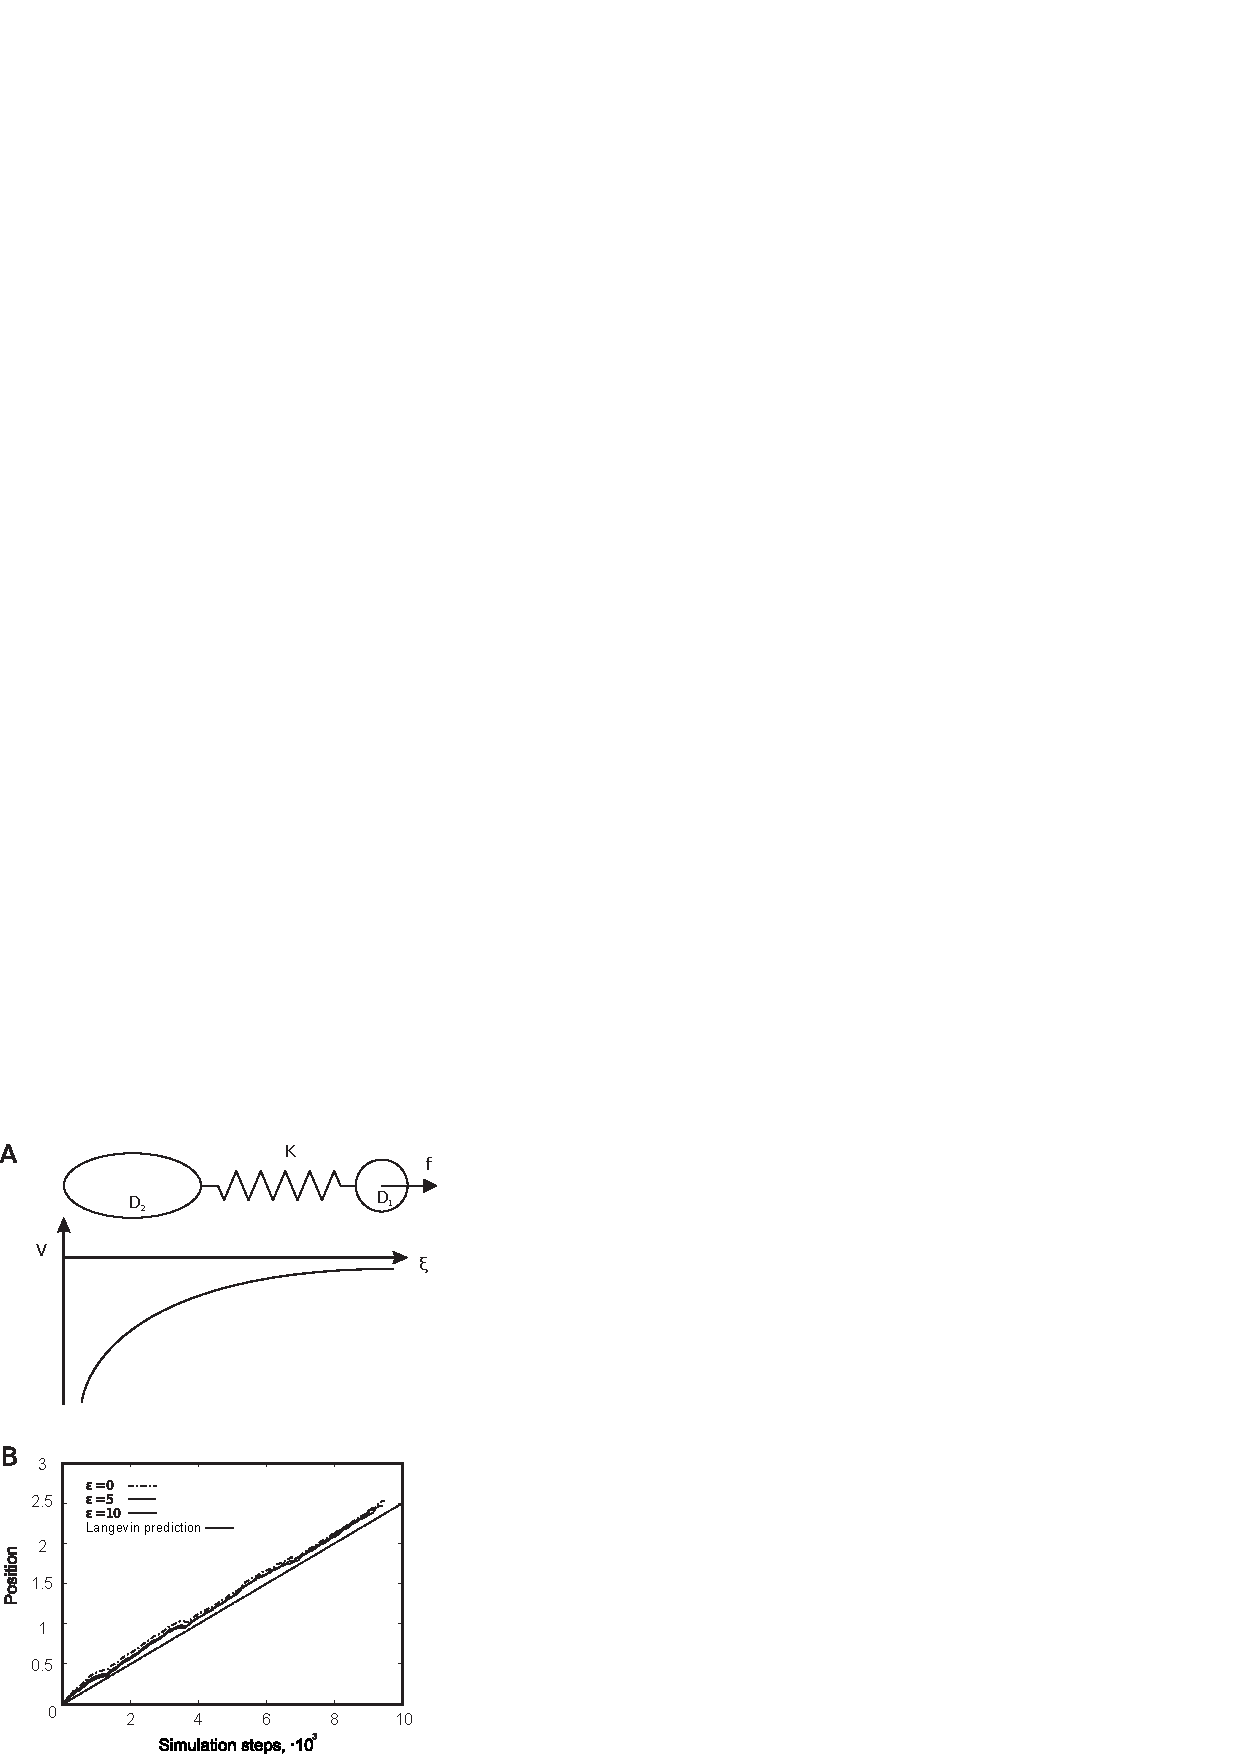
\includegraphics[scale=1.2]{../figures/langevin_spring.pdf}
\end{center}
 \caption[Drift of a particle together with the associated potential well]{Drift of a particle together with the associated potential well (from \cite{Kiselev2011}). (A) A sketch of the hypothetical system that consists of a particle (the peptide) that diffuses under the action of a force f while associated with a second particle (lipid shell) via the interaction potential $V$, symbolically depicted as a spring with constant K. (B) Results of 1D Monte-Carlo simulations for the system shown in A where $V$ is given by eq. \eqref{strange_potential}. All quantities are in arbitrary nondimensional units. Time has been rescaled by the Monte-Carlo acceptance rate as suggested in \cite{Sanz2010}.}
\label{fig:langevin_spring}
\end{figure}
The characteristic correlation time of the noise terms $\eta_{1,2}$ is of the same order as the unit time step of the MCA ($\sim1$ $\mu$s). However, the peptide drift in the MCA is considered at time scales of about 1000 time steps ($\sim1$ ms). Thus, at such large time scales the contribution of the noise terms $\eta_{1,2}$ in eqs. \eqref{Langevin_equations} can be neglected and the steady state value of $\xi$ can be calculated by the subtraction of the second equation from the first one:
\begin{equation}
\label{Langevin_subtraction}
 0 = \frac{d\xi}{dt} = \frac{f}{\gamma_1} - \Big(\frac{K}{\gamma_1} + \frac{K}{\gamma_2}\Big)\xi
\end{equation}

By rearranging of eq. \eqref{Langevin_subtraction} one can obtain the steady state value of $\xi$:
\begin{equation}
\label{equation_for_xi}
 \xi = \frac{f/\gamma_1}{K/\gamma_1 + K/\gamma_2}
\end{equation}

An expression, describing the behavior of $\zeta$, can be derived by adding together two equations in the system \eqref{Langevin_equations}:
\begin{equation}
\label{equation_for_zeta0}
  \frac{d\zeta}{dt} = \frac{f}{\gamma_1} + \Big(\frac{K}{\gamma_2} - \frac{K}{\gamma_1}\Big)\xi
\end{equation}

Using eq. \eqref{equation_for_xi} and taking into account that $\zeta/2$ represents the position of the center of mass of the two particles, the eq. \eqref{equation_for_zeta0} can be rewritten in the following form:
\begin{equation}
 \label{velocity_center_mass}
  2v = \frac{f}{\gamma_1} + \Big(\frac{K}{\gamma_2} - \frac{K}{\gamma_1}\Big)\frac{f}{\gamma_1}\frac{\gamma_1\gamma_2}{K(\gamma_1 + \gamma_2)}
\end{equation}
where $v$ is the velocity of the center of mass of the two particles. After rearranging of eq. \eqref{velocity_center_mass} the velocity has the following form:
\begin{equation}
 v= \frac{f}{\gamma_1+\gamma_2}
\end{equation}

Remembering Stokes-Einstein's relation:
\begin{equation}
 D_{1,2} = \frac{k_BT}{\gamma_{1,2}}
\end{equation}

one can obtain the final form of $v$:
\begin{equation}
 v=\frac{f}{k_BT}\frac{D_1D_2}{D_1+D_2}
\end{equation}

Therefore the velocity $v$ does not depend on the spring constant $K$. Illustrating this fact, Fig. \ref{fig:langevin_spring}, B, shows kinetic Monte-Carlo simulations of the system of two particles interacting via the sum of a spring and a finite-radius electrostatic potential $V'$ of variable size defined as follows:
\begin{equation}
\label{strange_potential}
 V'= \left\{
  \begin{array}{l l}
    \varepsilon r_0 \bigg[\frac{e^{-r/\lambda}}{r+r_0} - \frac{e^{-r_C/\lambda}}{r+r_0}\bigg], & \quad r>r_C \\
    0, & \quad r<r_C\\
  \end{array} \right.
\end{equation}
where $r_C=3\lambda$.

The most relevant prediction of this simplified model for the lateral dynamics of the peptide on the membrane is that a particle interacting with a lipid shell should move slower due to the combined drag term which is equal to $k_BT(D_1+D_2)/D_1D_2$. Therefore, any finite diffusivity of the lipid shell associated with the peptide will reduce the peptide effective mobility in the gradient of lipids. I believe that this effect could qualitatively explain the effective coefficient that was found in fitting the simulation results to the theory.





